\documentclass[tikz,border=10pt]{standalone}
\usepackage{tikz}
\usetikzlibrary{arrows.meta, positioning, shapes.geometric}

\begin{document}
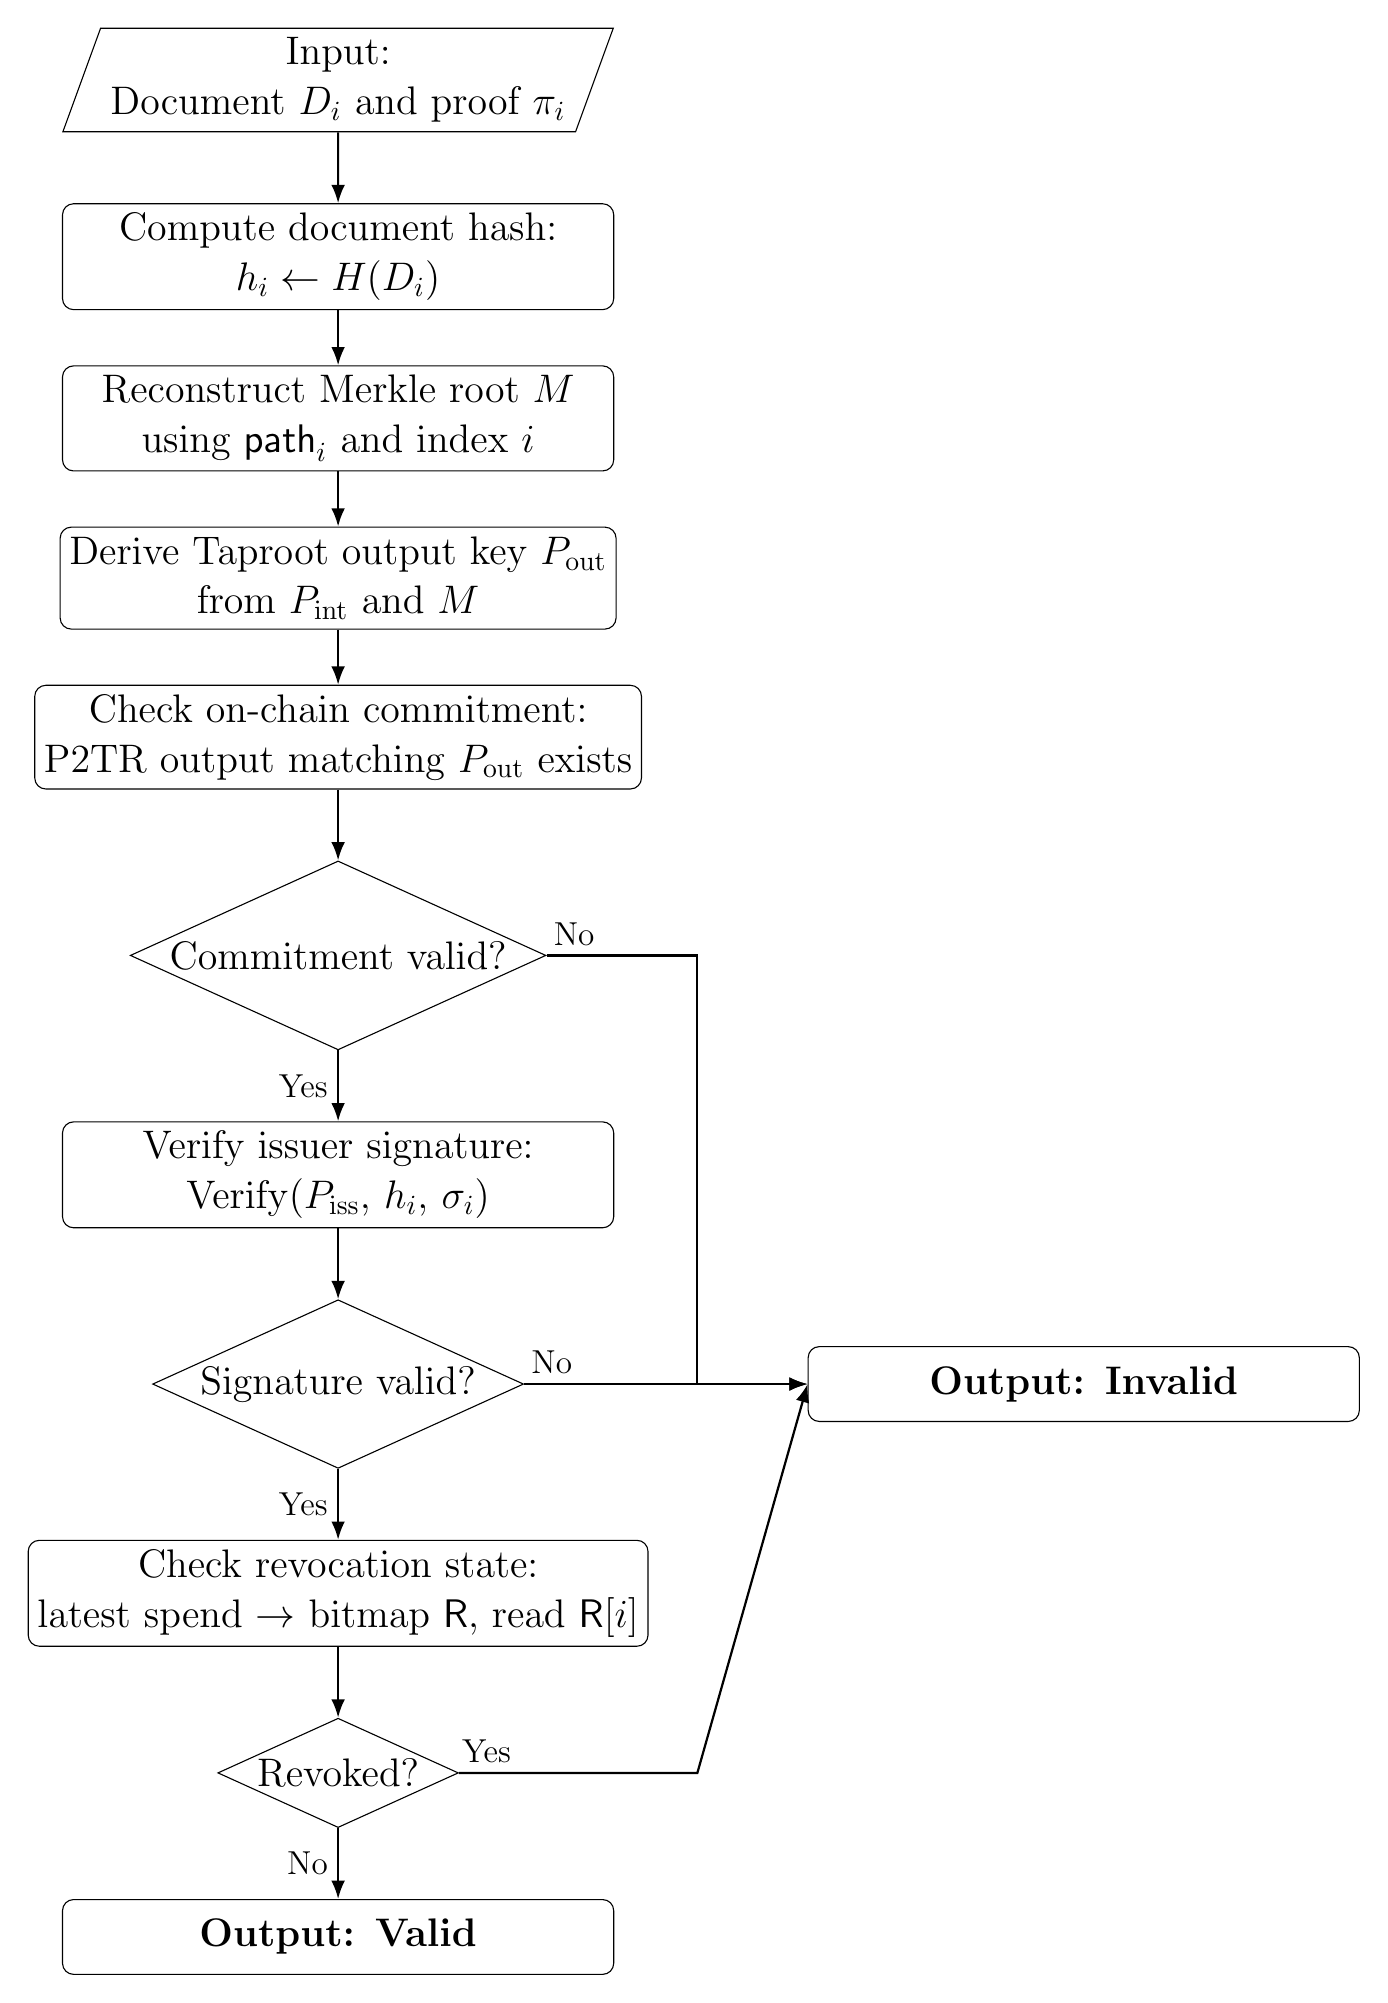
\begin{tikzpicture}[
    font=\Large,
    proc/.style={
        draw, rounded corners,
        align=center,
        minimum width=7.0cm,
        minimum height=0.95cm
    },
    io/.style={
        draw, trapezium,
        trapezium left angle=70,
        trapezium right angle=110,
        align=center,
        minimum width=7.0cm,
        minimum height=0.95cm
    },
    decision/.style={
        draw, diamond,
        aspect=2.2,
        align=center,
        inner sep=1pt
    },
    arrow/.style={-Latex, thick},
    note/.style={font=\large}
]

% ===== MAIN COLUMN =====
\node[io] (input) {Input:\\Document $D_i$ and proof $\pi_i$};

\node[proc, below=0.9cm of input] (hash)
{Compute document hash:\\$h_i \leftarrow H(D_i)$};

\node[proc, below=0.7cm of hash] (merkle)
{Reconstruct Merkle root $M$\\using $\mathsf{path}_i$ and index $i$};

\node[proc, below=0.7cm of merkle] (tap)
{Derive Taproot output key $P_{\mathrm{out}}$\\from $P_{\mathrm{int}}$ and $M$};

\node[proc, below=0.7cm of tap] (commit)
{Check on-chain commitment:\\P2TR output matching $P_{\mathrm{out}}$ exists};

\node[decision, below=0.9cm of commit] (d1) {Commitment valid?};

\node[proc, below=0.9cm of d1] (sig)
{Verify issuer signature:\\$\mathrm{Verify}(P_{\mathrm{iss}},\, h_i,\, \sigma_i)$};

\node[decision, below=0.9cm of sig] (d2) {Signature valid?};

\node[proc, below=0.9cm of d2] (rev)
{Check revocation state:\\latest spend $\rightarrow$ bitmap $\mathsf{R}$, read $\mathsf{R}[i]$};

\node[decision, below=0.9cm of rev] (d3) {Revoked?};

\node[proc, below=0.9cm of d3] (valid)
{\textbf{Output: Valid}};

% ===== INVALID NODE (RIGHT) =====
\node[proc, right=3.6cm of d2] (invalid)
{\textbf{Output: Invalid}};

% ===== FAILURE RAIL (INVISIBLE GUIDELINE) =====
% Place a fixed rail to the right of the decision stack.
% Adjust x-shift (2.2cm) if you want more spacing.
\coordinate (rail) at ([xshift=2.2cm]d2.east);

% ===== MAIN FLOW ARROWS =====
\draw[arrow] (input) -- (hash);
\draw[arrow] (hash) -- (merkle);
\draw[arrow] (merkle) -- (tap);
\draw[arrow] (tap) -- (commit);
\draw[arrow] (commit) -- (d1);

\draw[arrow] (d1) -- node[left, note]{Yes} (sig);
\draw[arrow] (sig) -- (d2);
\draw[arrow] (d2) -- node[left, note]{Yes} (rev);
\draw[arrow] (rev) -- (d3);
\draw[arrow] (d3) -- node[left, note]{No} (valid);

% ===== FAILURE ROUTING VIA RAIL (NO OVERLAPS) =====
% d1: No -> rail at d1 height -> rail down to d2 height -> invalid
\draw[arrow]
  (d1.east) -- ++(0.35,0) node[above, note]{No}
  -- ([yshift=0cm]rail |- d1.east)
  -- ([yshift=0cm]rail |- d2.east)
  -- (invalid.west);

% d2: No -> rail at d2 height -> invalid
\draw[arrow]
  (d2.east) -- ++(0.35,0) node[above, note]{No}
  -- ([yshift=0cm]rail |- d2.east)
  -- (invalid.west);

% d3: Yes -> rail at d3 height -> invalid
\draw[arrow]
  (d3.east) -- ++(0.35,0) node[above, note]{Yes}
  -- ([yshift=0cm]rail |- d3.east)
  -- (invalid.west);

\end{tikzpicture}
\end{document}
